\section{Facettentypen}
\label{sec:Konzeption:FacetTypes}

\begin{figure}[h]
    \myfloatalign
    \subfloat[Facettentyp String]{
        \label{fig:FacetTypes:subfloat:FacetType_String}
        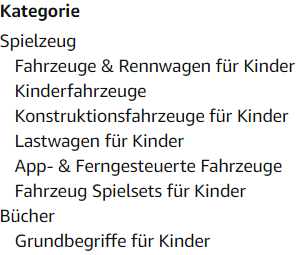
\includegraphics[width=.3\linewidth]{chapters/3_Konzeption/res/Facets/amazon_facet_search_string.png}
    }
    \subfloat[Facettentyp Number]{
        \label{fig:FacetTypes:subfloat:FacetType_Number}
        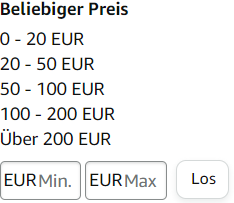
\includegraphics[width=.3\linewidth]{chapters/3_Konzeption/res/Facets/amazon_facet_search_number.png}
    }
    \subfloat[Facettentyp Boolean]{
        \label{fig:FacetTypes:subfloat:FacetType_Boolean}
        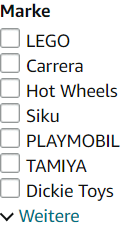
\includegraphics[width=.15\linewidth]{chapters/3_Konzeption/res/Facets/amazon_facet_search_boolean.png}
    }
    \caption{Von Amazon gegebene Facetten, mit eingegebenem Begriff ''Fahrzeug''}
    \label{fig:FacetTypes:Amazon_FacetTypes}
\end{figure}

Die in Abbildung \ref{fig:FacetTypes:Amazon_FacetTypes} gezeigten Facettentypen werden über Amazon bereitgestellt.
Diese sind aufteilbar in Zeichenketten (\ref{fig:FacetTypes:subfloat:FacetType_String}), Zahlen (\ref{fig:FacetTypes:subfloat:FacetType_Number}) und Booleans (\ref{fig:FacetTypes:subfloat:FacetType_Boolean}). Diese drei Typen stellen hierbei die primitiven Datentypen dar \cite{TODO primitivie Datentypen}, wobei Zahlen in ganze und rationale Zahlen unterschieden werden müssen.

Um diese Datentypen abzudecken, erstellen wir die Facettentypen ''Number'', ''String'' und ''Boolean''.
Hierbei müssen die Werte der Facetten mit ihrem jeweiligen Typen übereinstimmen. Das bedeutet, dass Zahlen als Facet\-ten\-wert zum ''Number''-Facetten\-typ gehören, eine Zeichen\-kette als Facetten\-wert zum ''String''-Facetten\-typ usw.
Zeichenketten können jedoch als Datum formatiert werden \cite{TODO Datums-Formatierung}, wodurch sie einen speziellen Typ annehmen können.
Aufgrund dessen sollte auch eine Facette des Types Datum verwendet werden.

Somit gilt:
\begin{description}
    \item[Number Facette:]
    Ein Facettenwert \(v_f\) in der Number Facette \(F_N\) ist eine Zahl oder kann mehrere Zahlen enthalten.
    \\Es gilt: \(\forall v_f \in F_N: v_f \in \mathbb{Q}\)
    \item[Boolean Facette:]
    Ein Facettenwert \(v_f\) in der Boolean Facette \(F_B\) ist entweder ein oder mehrere true oder false Werte.
    \\Es gilt: \(\forall v_f \in F_B: v_f \in \{true, false\}\)
    \item[String Facette:]
    Ein Facettenwert \(v_f\) in der String Facette \(F_S\) ist entweder ein oder mehrere Zeichenketten.
    \\Es gilt: \(\forall v_f \in F_S: v_f \in Alphabet\)
    \item[Date Facette:]
    Ein Facettenwert \(v_f\) in der Date Facette \(F_D\) ist ein Datum.
    \\Es gilt: \(\forall v_f \in F_D: v_f = DATUM\)
\end{description}

%%%%%%%%%%%%%%%%%%%%%%%%%%%%%%%%%%%%%%%%%%%%%%%%%%%%%%%%%%%%%%%%%%%%%%%%%%
\section{Facettenwert-Filterung}
\label{sec:Konzeption:FacetValue_filtering}
Facetten müssen zusätzlich zur Typisierung auch eine Filterung derer Werte aufweisen.
So sieht man beispielsweise in Abbildung \ref{fig:FacetTypes:subfloat:FacetType_Number} eine Bereichseingabe des Preises mit Minimum und Maximum.

Eine String-Facette, zu sehen in Abbildung \ref{fig:FacetTypes:subfloat:FacetType_String}, stellt ledigilich ein Label dar.
Man kann sie jedoch auch so gestalten, dass sie als Suchfunktion dargestellt werden kann. Somit können Nutzer Artikel oder Dokumente nach ihrer jeweiligen Facetten-Suchanfrage filtern.
Beispielsweise könnte man dann, anstelle die Kategorie anzuklicken, die jeweilige Kategorie eintippen.

Facetten des Typs Boolean können hingegen nur zwei mögliche Werte annehmen: Ausgewählt oder nicht ausgewählt, zu sehen in Abbildung \ref{fig:FacetTypes:subfloat:FacetType_Boolean}.

Facetten des Typs Datum können ein oder zwei verschiedene Daten annehmen.
Wird ein spezifisches Datum gewählt, so filtert man die Werte nach diesem einen spezifischen Datum,
werden hingegen zwei verschiedene Werte gewählt, so filtert man nach einem Bereich, der sich durch die zwei Daten ergibt.

Wird keine Facette ausgewählt, so werden alle Artikel/Dokumente angezeigt.

%%%%%%%%%%%%%%%%%%%%%%%%%%%%%%%%%%%%%%%%%%%%%%%%%%%%%%%%%%%%%%%%%%%%%%%%%%
\section{Facetten-IDs}
\label{sec:Konzeption:FacetIDs}
Facetten benötigen eine eindeutige Identifikation, damit diese nicht mehrmals generiert werden.
Semi-strukturierte Daten könnten eine eindeutige Zuweisung in einem extra Feld liefern. 
Da jedoch dynamisch erzeugte Facetten generiert werden und die semi-strukturierten Daten zufällig eingelesen und keinem bestimmten Schema folgen, können sie keine eindeutige Zuweisung liefern.
Jedoch können die jeweiligen Namen der Felder, innerhalb der Daten verwendet werden um einen einmaligen Identifikator zu erzeugen.

\begin{figure}[h]
    \myfloatalign
    \subfloat[JSON mit einem simplen Objekt]{
        \label{fig:facetIds:subfloat:jsonSingleObject}
        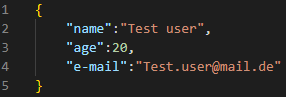
\includegraphics[width=.45\linewidth]{chapters/3_Konzeption/res/Facets/facetgeneration_json_singleObject.png}
    }\quad
    \subfloat[JSON mit einem verschachtelten Objekt]{
        \label{fig:facetIds:subfloat:jsonSingleNestedObject}
        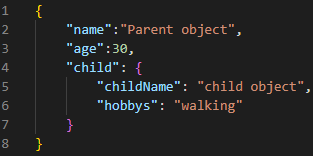
\includegraphics[width=.45\textwidth]{chapters/3_Konzeption/res/Facets/facetgeneration_json_singleObjectNested.png}
    }
    \caption{Darstellung zweier JSON-Objekte.}
    \label{fig:facetIds:jsonObjects}
\end{figure}

Die in Abbildung \ref{fig:facetIds:jsonObjects} gezeigten JSON-Dateien dienen als Darstellungsbeispiel.
Hierbei hat Abbildung \ref{fig:facetIds:subfloat:jsonSingleObject} die Felder: ''name'', ''age'' und ''e-mail'', aus denen die gleichnamigen Facetten generiert werden sollen.

Komplizierter wird es bei dem in Abbildung \ref{fig:facetIds:subfloat:jsonSingleNestedObject} gezeigten verschachtelten JSON-Objekt.
Hierbei gibt es das Feld ''child''. 
Dieses Feld enthält ein weiteres Objekt, mit weiteren Feldern, welche auch zur ID-Generierung in Betracht gezogen werden müssen. 
So sollen ''childName'' und ''hobbys'' auch als Facetten betrachtet werden.
Die IDs sollten hierbei eine Konkatination der Eltern-Facette und der Kind-Facette sein. Das Trennzeichen kann hierbei frei bestimmt werden.
So wären die folgenden IDs das Ergebnis aus der eben genannten Konkatination: ''child.childName'' und ''child.hobbys''.

Damit Nutzer spezifizierter eine Suche angehen können, werden die verschachtelten Facetten nicht zu bereits bestehenden Facetten, wie z.B. ''name'' und ''childName'' hinzugefügt, sondern separat betrachtet.